\documentclass[letterpaper,addpoints,answers]{exam}
\usepackage{graphicx}
\usepackage{multicol}
\usepackage{pgf}
\usepackage{tikz}
\usepackage{circuitikz}
\usetikzlibrary{arrows,shapes,trees}

\begin{document}

\begin{coverpages}
 \large\bfseries
 
 \noindent 
 Physics 252: Electronics
 
 \vspace{2ex}
 \noindent
 Final Exam: May 7, 2013

 \vspace{5ex}
 \noindent 
 Name:\enspace\makebox[2in]{\hrulefill}\\

 \vspace{5ex}
 \noindent 
 This test is administered under the rules and regulations of the honor 
 code of the College of William \& Mary.  

 \vspace{5ex}
 \noindent 
 \begin{itemize}
  \item Show your work, and \textbf{circle your answers}.
  \item You can use your notes, your lab book and the text book.
  \item The lecture slides or lab manuals are not allowed.
 \end{itemize}

 \vspace{5ex}
 \begin{center}
  \gradetable[v][questions]
 \end{center}
\end{coverpages}
 

\begin{questions}

\begin{question}
 Consider the circuit shown below:
 \begin{center}
  \begin{circuitikz}
   \draw (2.5,0) to[short,o-] (2,0) to[R,l=$R_3$] (0,0) to[battery,l=$V_b$] (0,2) to[R,l=$R_1$] (2,2) to[short,-o] (2.5,2)to[open,v^=$V_{out}$] (2.5,0);
   \draw (0,2) to[R,l=$R_2$,*-*] (2,0);
  \end{circuitikz}
 \end{center}
 where $R_1 = 8$\,k$\Omega$, $R_2 = 6$\,k$\Omega$, $R_3 =3$\,k$\Omega$, and the battery voltage $V_b = 18$\,V.
 
 \emph{Hint 1:} For solving the problems below, it may be helpful to mentally connect a dummy load and express symbolically the $V_{out}$ versus $I_{out}$ for different load resistors $R_L$.
 \emph{Hint 2:} There is also a faster way.
 \begin{parts}
  \part[8]
  What is the Th\'{e}venin voltage  of this circuit?

  \vskip 1.75in
  \part[8]
  What is the Th\'{e}venin resistance  of this circuit?

  \vskip 1.75in
  \part[5]
  If someone connected a load with resistance $R_L = 1$\,k$\Omega$, what is the power dissipated by this load?

  \vskip 0.5in
  \part[4]
  While the same load is connected to the circuit, what is the total power dissipated by all resistors (excluding the load)  of the circuit network.

  \vskip 0.5in
 \end{parts}
\end{question}

\pagebreak

\begin{question}
 Consider the bridged T-filter shown below.  The input comes in from the left and the output is taken from the right.  
 
 \emph{Hint 1:} You may find it useful to use the Kirchhoff rules to analyze this problem. \emph{Hint 2:} There is also a faster way.
 \begin{center}
  \begin{circuitikz}
   \draw (-2,4) node[anchor=east]{$v_{in}$} to[short,o-*] (-1.5,4) to[R,l=$2R$] (1.5,4) to[short,*-o] (2,4) node[anchor=west]{$v_{out}$};
   \draw (-1.5,4) to[short] (-1.5,3) to[C,l=$C$] (0,3) to[C,l=$C$] (1.5,3) to[short] (1.5,4);
   \draw (0,3) to[R, l=$R/2$, *-] (0,1) node[ground]{};
  \end{circuitikz}
 \end{center}
 \begin{parts}
  \part[4]
   What is the magnitude of the gain of this circuit for very low frequencies?
   \vskip 1.5in
  \part[4]
   What is the magnitude of the gain of this circuit for very high frequencies?
   \vskip 1.5in
  \part[2]
   What type of filter is this?
   \vskip 1.0in
\pagebreak
  \part[10]
   What is the gain of this circuit as a function of frequency?
   \vskip 2.0in
%   \part[4]
%    At what frequency does the gain have a minimum?
%    \vskip 2.0in
 \end{parts}
\end{question}

\pagebreak

\begin{question}
 A circuit consists of a battery of constant voltage (2.0\,V), two unknown components and a switch. The switch is closed at $t = 0$ and the output voltage across circuit element B is measured as a function of time.
 \begin{multicols}{2}
  \begin{center}
   \begin{circuitikz}[scale=1.5]
    \draw (0,0) node[ground]{} to[battery,l=$V$] (0,2) to[closing switch,l=switch] (1,2) to[generic,l=A] (3,2) to[short,-o] (3.5,2);
    \draw (0,0) to[short] (3,0) to[short,-o] (3.5,0);
    \draw (3,0) to[generic,l=B,*-*] (3,2);
    \draw (3.5,0) to[open,v>=$v_{out}$] (3.5,2);
   \end{circuitikz}
  \end{center}
 \columnbreak
  \begin{center}
   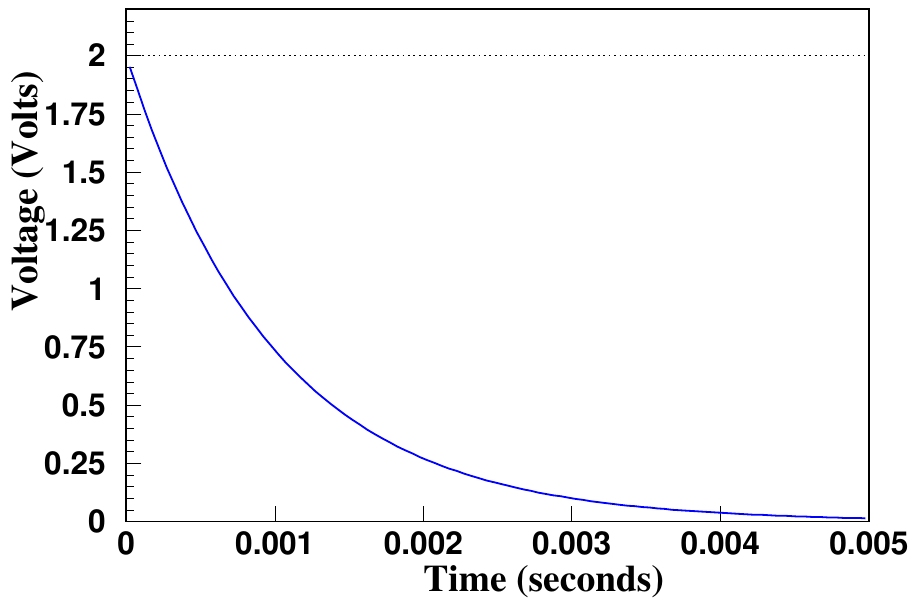
\includegraphics[width=0.45\textwidth]{images/exponential_decay}
  \end{center}
 \end{multicols}
 \begin{parts}
  \part[3]
  What is the characteristic time (approximately) of the circuit?
  \vskip 1in
  \part[4]
  Sketch the voltage across circuit element A as a function of time.
  \vskip 2in
  \part[10]
  Draw the diagram for at least two different circuits that can produce the observed behavior.  In this context ``different circuits'' have at least one component of a different type, so not just a change in their values.
  \vskip 2.5in
  \part[8]
  With an ohmmeter you measure the equivalent resistance of the two elements as combined in series and you find a value of 100\,$\Omega$.  Which of the two circuits is correct, and what are the two components, including their values?
  \vskip 2.5in
 \end{parts}
\end{question}

\pagebreak

\begin{question}
 Consider the diagram shown below with a sinusoidal input signal $v_{in}$ with an amplitude of 0.01\,V and $V_{CC} = 15 V$.
 \begin{center}
  \begin{circuitikz}
   \draw (4,4) node[npn](npn1){} node{$T_1$};
   \draw (8,5) node[npn](npn2){} node{$T_2$};
   \draw (0,4) node[anchor=east]{$v_{in}$} to[C,l=$C_1$,o-*] (2,4) to[short] (npn1.B);
   \draw (npn1.E) -| (4,3);
   \draw (4,3) to[short,*-] (3,3) to[R,l=$R_E$,-*] (3,1);
   \draw (4,3) to[short,*-] (4.5,3) to[C,l=$C_E$,-*] (4.5,1);
   \draw (2,1) to[R,l=$R_2$] (2,4) to[R,l=$R_1$] (2,7) to[short] (4,7) to[short] (6,7) -| (npn2.C);
   \draw (4,7.5) node[anchor=south]{$V_{CC}$} to[short,o-*] (4,7) to[R,l=$R_C$,*-] (npn1.C) |- (4,5) to[C,l=$C_2$,*-*] (6,5) to[short] (npn2.B);
   \draw (6,7) to[R,l=$R_3$,*-*] (6,5) to[R,l=$R_4$,*-*] (6,1);
   \draw (npn2.E) |- (8,4) to[C,l=$C_3$,*-o] (10,4) node[anchor=west]{$v_{out}$};
   \draw (2,1) to[short] (4.5,1) node[ground]{} to[short] (6,1) to[short] (8,1) to[R,l=$R_e$,-*] (8,4);
  \end{circuitikz}
 \end{center}
 \begin{parts}
  \part[10]
  What does this circuit do?  Identify any subcircuits that perform separate functions.
  \vskip 5in
  \part
  \begin{subparts}
   \subpart[5]
   Explain the purpose of the three capacitors $C_1$, $C_2$ and $C_3$.
   \vskip 1.5in
   \subpart[5]
   Explain the purpose of the capacitor $C_E$.
   \vskip 1.5in
  \end{subparts}
  \part[5]
  Which values would you pick for $R_1$, $R_2$, $R_C$, $R_E$, $R_3$ and $R_4$ to achieve an amplification factor of at least 100?
  \vskip 2in
 \end{parts}
\end{question}

\pagebreak

% \begin{question}
%  Consider the non-inverting amplifier diagram shown below:
%  \begin{center}
%   \begin{circuitikz}
%    \draw (3,0.5) node[op amp](opamp){ } node[left=0.1] {$A$};
%    \draw (0,1) node[ground]{} to[R,l=$R_1$,-*] (opamp.-) |- (2.25,2) to[R,l=$R_2$] (3.75,2) -| (opamp.out);
%    \draw (1.5,0) node[anchor=east]{$v_{in}$} to[short,o-] (opamp.+);
%    \draw (opamp.out) to[short,*-] (4.5,0.5) node[anchor=west]{$v_{out}$};
%   \end{circuitikz}
%  \end{center}
%  \begin{parts}
%   \part[10]
%   Find the expression for the output voltage $v_{out}$ in terms of $v_{in}$, $R_1$, $R_2$, and $A$. Do \textbf{not} assume that $A$ is infinite.
%   \vskip 2.5in
%   \part
%   The gain of an op amp typically falls off by 20\,dB per decade in frequency, in other words the product of gain and bandwidth is constant.  Assume that the gain-bandwidth product is $A(f) \times f = 10$\,MHz and the resistor ratio is $R_2 / R_1 = 10$.
%   \begin{subparts}
%    \subpart[5]
%    What is the gain of the system at 10~Hz?
%    \vskip 0.6in
%    \subpart[5]
%    What is the gain of the system at 10~MHz?
%    \vskip 0.6in
%   \end{subparts}
%   \part[5]
%   Consider the practical limitations now.  If  $R_2 / R_1 = 99$, $v_{in} = 0.01$\,V, and $A = \infty$, but the maximum output current of the op amp is 2\,mA.  What is the smallest possible load resistor that you can connect to the output without overloading the op amp?  Assume that $R_2 \gg R_L$.
%   \vskip 0.5in
%   \bonuspart[5]
%   What is the output impedance of this amplifier at low frequencies?  \textbf{Why} do you think so?  Assume $A = \infty$.
%   \vskip 0.4in
%  \end{parts}
% \end{question}
% 
% \pagebreak

\begin{question}
 Consider the two modified non-inverting amplifier diagrams shown below:
 \begin{multicols}{2}
  \begin{center}
   \begin{circuitikz}
    \draw (3,0.5) node[op amp](opamp){} node[left=0.1] {$A$};
    \draw (0,1) node[ground]{} to[R,l=$R_1$,-*] (opamp.-) |- (2.25,2) to[R,l=$R_2$] (3.75,2) -| (opamp.out);
    \draw (1.5,0) node[anchor=east]{$v_{in}$} to[short,o-] (opamp.+);
    \draw (opamp.out) to[short,*-] (4.5,0.5) to[R,l=$R_3$] (6.5,0.5) node[anchor=west]{$v_{out}$};
   \end{circuitikz}
  \end{center}
 \columnbreak
  \begin{center}
   \begin{circuitikz}
    \draw (3,0.5) node[op amp](opamp){} node[left=0.1] {$A$};
    \draw (0,1) node[ground]{} to[R,l=$R_1$,-*] (opamp.-) |- (2.25,2) to[R,l=$R_2$] (3.75,2) -| (6.0,0.5);
    \draw (1.5,0) node[anchor=east]{$v_{in}$} to[short,o-] (opamp.+);
    \draw (opamp.out) to[R,l=$R_3$] (6.0,0.5) to[short,*-] (6.5,0.5) node[anchor=west]{$v_{out}$};
   \end{circuitikz}
  \end{center}
 \end{multicols}
 Assume that all op amps are ideal (with open loop gain $A = \infty$).
 \begin{parts}
  \part
   Consider the diagram on the left (resistor in output only).
   \begin{subparts}
    \subpart[2]
    Express $v_{out}$ as a function of $v_{in}$ and circuit components assuming no load is connected.
    \vskip 1.4in
    \subpart[4]
    Express $v_{out}$ as a function of $v_{in}$ and circuit components when a dummy load $R_L$ is connected.
    \vskip 1.4in
    \subpart[4]
    Determine the output impedance of the circuit.
    \vskip 1.4in
   \end{subparts}
  \part
   Consider the diagram on the right (resistor in feedback and output).
   \begin{subparts}
    \subpart[2]
    Express $v_{out}$ as a function of $v_{in}$ and circuit components assuming no load is connected.
    \vskip 1.4in
    \subpart[4]
    Express $v_{out}$ as a function of $v_{in}$ and circuit components when a dummy load $R_L$ is connected.
    \vskip 1.4in
    \subpart[4]
    Determine the output impedance of the circuit.
    \vskip 1.4in
   \end{subparts}
 \end{parts}

\end{question}

\pagebreak

\begin{question}
 \begin{parts}
  \part[20]
  Design (using as many op amps as needed) and sketch a circuit with an output that is governed by the following expression:
  \begin{equation}
   V_{out} = -5(V_1+ V_2) + 10 V_3.
  \end{equation}
  Explain your design.  Specify all relevant components values.  Assume that you are using ideal op amps (with open loop gain $A = \infty$).
  \bonuspart[5]
  Bonus points if you use only one op amp.
  \vskip 2.5in
 \end{parts}
\end{question}
\pagebreak



\end{questions}

\end{document}
